% Chapter 3

\chapter{Geles polim\'ericos} % Main chapter title

\label{Chapter3} % For referencing the chapter elsewhere, use \ref{Chapter1} 

%----------------------------------------------------------------------------------------

% Define some commands to keep the formatting separated from the content 
\newcommand{\keyword}[1]{\textbf{#1}}
\newcommand{\tabhead}[1]{\textbf{#1}}
\newcommand{\code}[1]{\texttt{#1}}
\newcommand{\file}[1]{\texttt{\bfseries#1}}
\newcommand{\option}[1]{\texttt{\itshape#1}}

%----------------------------------------------------------------------------------------

\section{Modelo sencillo: 2 fases}

Los microgeles son part\'iculas blandas hechas de cadenas de pol\'imeros reticulados que pueden mostrar un comportamiento tanto coloidal como macromolecular \addcite[plamper2017,lyon2012].
Inmersas en soluciones acuosas, estas part\'iculas incorporan y retienen grandes cantidades de agua dentro de su estructura polim\'erica.
Por lo general, sus di\'ametros van desde decenas de nan\'ometros (nanogeles) hasta varias micras.
Sin embargo, la caracter\'istica m\'as llamativa de estas part\'iculas es su capacidad para absorber o liberar solventes y cambiar de tama\~no en respuesta a una variedad de est\'imulos externos.
Este comportamiento de respuesta es reversible y depende de la composici\'on qu\'imica de la red polim\'erica.


Los microgeles compuestos por cadenas polim\'ericas que tienen segmentos \'acidos como el \'acido acr\'ilico o metacr\'ilico (AA y MAA, respectivamente) se hinchan/deshinchan muchas veces en respuesta a cambios en el pH de la soluci\'on \addcite[snowden1996,Zhou1998].
El pH particular que marca el inicio y caracteriza esta transici\'on es el pKa aparente del microgel, que depende de la concentraci\'on de sal de la soluci\'on y frecuentemente difiere del pKa intrínseco del mon\'omero \'acido.
Estos microgeles tambi\'en ajustan su tama\~no en respuesta a cambios en la concentraci\'on de sal de la soluci\'on \addcite[snowden1996].

An\'alogamente, los microgeles de algunos pol\'imeros termosensibles experimentan una transici\'on de fase de volumen (VPT) cuando se calientan por encima de una temperatura caracter\'istica (VPTT o $T_{pt}$)\addcite[Pelton1986,Pelton2000].
Este comportamiento se origina porque tales pol\'imeros son insolubles en agua por encima de cierta temperatura de soluci\'on cr\'itica m\'as baja (LCST) \addcite[Kawaguch2020].
Normalmente, la LCST del pol\'imero y la VPTT de la red reticulada son aproximadamente id\'enticas. 
Este es el caso de las part\'iculas de microgel de poli(N-isopropilacrilamida) (PNIPAm) \addcite[Pelton1986], cuyo volumen colapsa por encima de $32 C$, el LCST del pol\'imero lineal \addcite[Schild1992].

Al tener un VPTT alrededor de la temperatura corporal, los microgeles de PNIPAm han generado un gran inter\'es para aplicaciones biom\'edicas \addcite[Guan2011].
Las estrategias para controlar el VPTT de los microgeles incluyen la s\'intesis de nuevos mon\'omeros termosensibles\addcite[Cai2007, Macchion2019], as\'i como la copolimerizaci\'on con un mon\'omero i\'onico o ionizable \addcite[Hirose1987, Lopez2010].
Este \'ultimo enfoque produce microgeles de respuesta m\'ultiple que son susceptibles a cambios en la temperatura, el pH y la concentraci\'on de sal \addcite[snowden1996, Farooqi2017].
Los microgeles de NIPAm y AA han sido ampliamente estudiados \addcite[Morris1997, Jones2000, Bradley2005, Begum2016];
Tambi\'en se han investigado microgeles de copol\'imeros de NIPAm y MAA \addcite[Dowding2000, Hoare2004, Giussi2015].
El VPTT de estos microgeles de respuesta m\'ultiple depende del pH de la soluci\'on y la concentraci\'on de sal, y la fracci\'on de mon\'omero ionizable en las cadenas de pol\'imero \addcite[Morris1997, Jones2000, Hoare2004, Bradley2005, Lee2008, Wong2009, Hamzavi2016].
Adem\'as, la incorporaci\'on del comon\'omero \'acido proporciona un mecanismo controlado por el pH para la captaci\'on/liberaci\'on de mol\'eculas con carga opuesta, lo que hace que los microgeles de respuesta m\'ultiple sean atractivos para el dise\~no de sistemas funcionales de administraci\'on de f\'armacos \addcite[Liu2017].

Las aplicaciones basadas en microgeles polim\'ericos son cada vez m\'as diversas y cada vez m\'as importantes en diferentes \'areas de la tecnolog\'ia \addcite[plamper2017].
Los nanocompuestos hechos de microgeles de poli(NIPAm-\emph{co}-MAA) que incorporan nanopart\'iculas de oro o plata o redes metal organicas tienen aplicaciones potenciales en el desarrollo de materiales con actividad catal\'itica  para la degradación de contaminantes industriales \addcite[Khan2013, Shi2014, Allegretto2020].
Estos microgeles tambi\'en se pueden aplicar para el desarrollo de emulsiones sensibles al pH, la sal y la temperatura \addcite[Ngai2005, Ngai2006, Brugger2008, Schmidt2011] o como plantillas para el ensamblaje de nanomateriales \addcite[Wong2009].
Los geles polim\'ericos de tama\~no nano/micro de respuesta m\'ultiple son excelentes candidatos para el desarrollo de aplicaciones biom\'edicas m\'inimamente invasivas, incluida la ingeniería de tejidos \addcite[Daly2020].
\addcite[citet:Culver2017A] han utilizado nanogeles de poli(NIPAm-co-MAA) funcionalizados para la uni\'on y detecci\'on de diferentes prote\'inas.
Recientemente se investigaron dispositivos basados en microgeles de poli(NIPAm-co-MAA) para la encapsulación/liberaci\'on del f\'armaco quimioterap\'eutico Doxorrubicina \addcite[Giussi2020, MartinesMoro2020, Pergushov2020].

En este contexto, en este cap\'itulo mostramos el desarrollo de una teor\'ia de equilibrio de dos fases y realizamos una investigaci\'on sistem\'atica del comportamiento termodin\'amico de microgeles compuestos de copol\'imeros aleatorios de NIPAm y un comon\'omero \'acido (MAA).
Este modelo describe la qu\'imica f\'isica detr\'as de todos los siguientes fen\'omenos: el hinchamiento del microgel impulsado por el pH, la dependencia no monot\'onica del tama\~no de part\'icula de la concentraci\'on de sal y el colapso de la red al aumentar la temperatura por encima del VPTT.
Nuestras predicciones brindan una imagen clara de los efectos de la composici\'on de la soluci\'on (pH, concentración de sal) y la qu\'imica del pol\'imero (contenido de MAA, grado de entrecruzamiento) en el VPT.
Tambi\'en investigamos las mejores condiciones para la encapsulaci\'on de doxorrubicina y daunorrubicina dentro de estos microgeles.
Los c\'alculos  ac\'a mostrados son espec\'ificos para el \'acido metacr\'ilico con $pKa = 4,65$, pero el comportamiento fisicoqu\'imico informado puede describir cualitativamente una variedad de microgeles basados en NIPAm que se han modificado con otros monómeros \'acidos que tienen diferente pka y diferente solubilidad a pH bajo.


El comportamiento de los microgeles de poli(NIPAm-co-MAA), incluido su VPT y la interacci\'on con pol\'imeros de carga opuesta, se ha descrito utilizando una variedad de t\'ecnicas experimentales \addcite[Hoare2004,Dowding2000, Kleinen2008, Kleinen2010, Giussi2015, Su2016, Giussi2020].
Tambi\'en se han aplicado teor\'ias  y simulaciones moleculares de grano grueso para investigar el comportamiento de los microgeles polim\'ericos sensibles a est\'imulos \addcite[quesada2011gel, ahualli2016coarse, Landsgesell2019SM].
Estos trabajos se han centrado principalmente en el hinchamiento y otras propiedades de las part\'iculas que tienen una red de pol\'imero permanentemente cargada , y algunos han abordado el efecto de la temperatura y la calidad del solvente \addcite[Jha2011,QuesadaPerez2013,QuesadaPerez2014,moncho-jorda2016a,ahualli2016coarse,AdroherBenitez2017PCCP].
Recientemente, estudios  con simulaciones han considerado la respuesta al pH de microgeles compuestos de pol\'imeros reguladores de carga\addcite[Schroeder2015, Rudov2017, Sean2018, Hofzumahaus2018, Lu2019].
Sin embargo, solo unos pocos trabajos te\'oricos han investigado las propiedades de los microgeles de respuesta m\'ultiple en funci\'on de la temperatura, el pH y la concentración de sal \addcite[CaprilesGonzalez2008, polotsky2013collapse].


\subsection{Fase Microgel}\label{sec:theory}
%%%%%%%%%%%%%%%%%%%%%%%%%%%%%%%%%%%%%%%%%%%%%%%%%%%%%%%%%%%%%%%%%%%%%


Consideremos un modelo de dos fases: un microgel de poli(NIPAm-\emph{co}-MAA) (P(NIPAm-MAA)) (fase $1$, denotada por $MG$) en contacto con una soluci\'on acuosa ( fase $2$, denotada por $s$).
Externamente, podemos controlar la temperatura $T$, el pH y la concentraci\'on de sal de esta soluci\'on, lo que da como resultado que el microgel tenga un radio $R$ y un volumen $V=\frac{4}{3}\pi R^3$.
El potencial termodin\'amico cuyo m\'inimo produce las condiciones de equilibrio dentro de la fase de microgel es el semi-gran potencial can\'onico, $\Omega_{MG}$, que contiene las siguientes contribuciones:
%
\begin{align}
    \begin{aligned}
       \Omega_{MG}=& -TS_{mix} + F_{chem,MAA} +  F_{ela}\\
       & + U_{elec}+  U_{ste} + U_{VDW} -{\sum_{\gamma}
        {\mu_\gamma N_\gamma}}
    \end{aligned}
    \label{eq:free-energy-implicit}
\end{align}
%

\noindent donde $S_{mix}$ es la entropí\'i de traslaci\'on (mezcla) de las especies libres en la fase de microgel: mol\'eculas de agua ($w$), hidronio ($H_3O^+$) e iones de hidr\'oxido ($OH^-$ ), y cationes de sal ($+$) y aniones ($-$).
Aqu\'i consideramos una sal monovalente, $KCl$, y asumimos que est\'a completamente disociada en iones de potasio y cloruro.
$F_{chem,MAA}$ es la energ\'ia química libre que describe la protonación de equilibrio de las unidades MAA.
$F_{ela}$ es la energía libre el\'astica que explica la libertad conformacional de la red polim\'erica.
$U_{elec}$ y $U_{ste}$ representan respectivamente las interacciones electrost\'aticas y las repulsiones est\'ericas.
$U_{VDW}$ es la contribuci\'on que describe las interacciones efectivas pol\'imero-disolvente; incorpora la transici\'on hidrofílica-hidrof\'obica de NIPAm al aumentar la temperatura por encima de su LCST.
Finalmente, la suma de $\gamma$ expresa el equilibrio qu\'imico con la fase de soluci\'on, donde $\mu_\gamma$ y $N_\gamma$ son el potencial qu\'imico y el n\'umero de mol\'eculas de la especie $\gamma$, respectivamente.
Aqu\'i, el subíndice $\gamma$ es  sobre las especies qu\'imicas libres, $\gamma \in \left\{ w, H_3O^+, OH^-, +,- \right\}$.
Hay que tener en cuenta que $\Omega_{MG}$ es un potencial semi grancan\'onico porque la fase de microgel puede intercambiar cada una de estas mol\'eculas con la fase de soluci\'on, mientras que la red de pol\'imero está confinada dentro de la primera.

La forma expl\'icita del potencial termodin\'amico es:




%
\begin{align}
\begin{aligned}
\beta&\frac{\Omega_{MG}(R)}{V}=\\& ~ \sum_{\gamma} \rho_\gamma\left(\ln\left(\rho_\gamma v_w\right) -1 + \beta\mu^0_\gamma\right) \\
& + \frac{\phi_{MAA}}{v_{MAA}} \left[f(\ln f+ \beta\mu^0_{MAA^-})\right.\\
&\qquad\left.+(1-f)(\ln (1-f)+\beta\mu^0_{MAAH})\right] \\
%
& +  \left(\sum_{\gamma } {\rho_\gamma q_\gamma + f\dfrac{\phi_{MAA}}{v_{MAA}}q_{MAA}}\right)\beta\psi_{MG}\\
%
& -\sum_{\gamma }{\rho_\gamma\beta\mu_\gamma}
 -\beta\mu_{H^+}(1-f)\dfrac{\phi_{MAA}}{v_{MAA}}\\
%
& + \chi (T, \phi_{NIPAm})\rho_w \phi_{NIPAm} \\
%
& + \dfrac{3}{2}\dfrac{N_{seg}}{n_{ch} V}\left[\left(\dfrac{R}{R_0}\right)^2 - \ln\dfrac{R}{R_0} -1\right]
%
\end{aligned}
\label{eq:free-energy}
\end{align}

\noindent donde el primer t\'ermino (segunda l\'inea) de $S_{mix}$; $\beta=\frac{1}{k_BT}$ y $k_B$ es la constante de Boltzmann.
La densidad num\'erica de la especie $\gamma$ es $\rho_\gamma$ y $\mu^0_\gamma$ es su potencial qu\'imico est\'andar, que tambi\'en se incluye en esta primera contribución; $v_w$ es el volumen de una mol\'ecula de agua.


La segunda y tercera l\'inea de la ec. \ref{eq:free-energy} (lado derecho) incorporan el equilibrio \'acido-base de las unidades MAA, donde $\phi_{MAA}$ es la fracci\'on de volumen que ocupan estos segmentos, $v_{MAA}$ es la volumen de este segmento, y $f$ es el grado de disociaci\'on o la fracci\'on de estas unidades que se cargan.
La fracci\'on de volumen de los segmentos MAA cargados es $f\phi_{MAA}$, y la de las unidades protonadas o sin carga es $(1-f)\phi_{MAA}$.
Los potenciales qu\'imicos est\'andar son $\mu^0_{MAA^-}$ y $\mu^0_{MAAH}$ para las especies cargadas y protonadas, respectivamente.
Hay qye tener en cuenta que aqu\'i usamos el t\'ermino segmento para identificar las unidades qu\'imicas (monómeros) que componen las cadenas polim\'ericas (MAA y NIPAm).


La siguiente contribuci\'on a la ec. \ref{eq:free-energy} es la energ\'ia electrost\'atica, donde $q_\gamma$ y $q_{MAA}$ son la carga el\'ectrica de las moléculas $\gamma$ y los segmentos MAA, respectivamente.
El potencial electrost\'atico dentro de la fase de microgel es $\psi_{MG}$.


La siguiente contribución (l\'inea 6 de eq.\ref{eq:free-energy}) refuerza el equilibrio qu\'imico entre el microgel y la fase de soluci\'on, donde el segundo t\'ermino representa esos protones unidos a unidades MAA sin carga;
a saber, $\mu_{H^+}\equiv\mu_{H_3O^+}$ se conjuga con el n\'umero total de protones,
$N_{H_3O^+}+N_{MAAH}=V\left(\rho_{H_3O^+}+(1-f)\dfrac{\phi_{MAA}}{v_{MAA}}\right)$.


El siguiente t\'ermino en el potencial termodin\'amico explica la respuesta de PNIPAm a los cambios de temperatura a trav\'es de un par\'ametro de interacci\'on pol\'imero solvente, $\chi$, que depende de la temperatura y la fracci\'on de volumen de NIPAm, $\phi_{NIPAm}$.
Seg\'un \addcite[afroze2000], este par\'ametro de Flory-Huggins se puede expresar como:
%
%


\begin{align}
\begin{aligned}
\chi (T, \phi_{NIPAm}) &=g_0(T) +g_1(T)\phi_{NIPAm} \\
 &~+ g_2(T)\phi_{NIPAm}^2
\end{aligned}
\end{align}

\noindent con
%
%
\begin{align}
\begin{aligned} 
g_k(T)=g_{k0} + \frac{g_{k1}}{T} + g_{k2}T
\end{aligned}
\end{align}


\noindent para  $k=0,1,2$, los coeficinetes son: $g_{00}= -12.947$, $g_{02}=0.044959\,$K$^{-1}$, $g_{10}= 17.920$, $g_{12}= -0.056944$\,K$^{-1}$, $g_{20}= 14.814$, $g_{22}= -0.051419$\,K$^{-1}$  y $g_{k1}\equiv 0$ \addcite[afroze2000]. 


El \'utimo t\'ermino en eq. \ref{eq:free-energy} es la contribuci\'on resultante de la elasticidad de la red de pol\'imero entrecruzado que forma la columna vertebral del microgel.
Esta expresi\'on se describe en \addcite[mocho-jorda2016a] y proviene del modelo de elasticidad del caucho,
donde $N_{seg}$ es el n\'umero total de segmentos en la red de pol\'imero y $n_{ch}$ es el n\'umero de segmentos por cadena de pol\'imero o \emph{longitud de cadena}.
Se tiene en cuenta que la constante de resorte en la energ\'ia libre el\'astica es proporcional al cociente $\dfrac{N_{seg}}{n_{ch}}$, que representa el n\'umero (total) de cadenas de pol\'imero en el microgel.
El radio del microgel seco es $R_0$, lo que satisface con la expresi\'on:

%
%
\begin{align}
\begin{aligned} 
\dfrac{4}{3}\pi R_0^3=V_0&=N_{seg}\Big( x_{MAA} v_{MAA}\\
&\qquad+x_{NIPAm} v_{NIPAm}\Big)
\end{aligned}
\end{align}


\noindent donde $V_0$ es el volumen de la part\'icula seca; $x_{MAA}$ y $x_{NIPAm}$ son la fracci\'on de los segmentos MAA y NIPAm, respectivamente.
Entonces, el n\'umero total de segmentos MAA es $x_{MAA}N_{seg}$ y el de unidades NIPAm es $x_{NIPAm}N_{seg}$, cada uno con un volumen $v_{NIPAm}$.
Los microgeles que consideramos aqu\'i satisfacen $x_{NIPAm}=1-x_{MAA}$.


Deben imponerse dos restricciones f\'isicas al potencial termodin\'amico dado por la ec. \ref{eq:free-energy}.
El volumen del microgel est\'a completamente ocupado por los segmentos de la red y las especies quí\'icas libres.
Esta restricci\'on de incompresibilidad incorpora las repulsiones est\'ericas (volumen excluido) y se puede expresar como:
%

%
%
\begin{align}
\begin{aligned}
\sum_{\gamma } \rho_\gamma v_\gamma  + \phi_{MAA} + \phi_{NIPAm} = 1
\end{aligned}
\label{eq:packing}
\end{align}



\noindent donde $v_\gamma$  es el volumen molecular de la especie $\gamma$, y la fracci\'on de volumen de cada componente de la red son: 
%
%
\begin{align}
\phi_{MAA}&=N_{seg}\dfrac{x_{MAA}v_{MAA}}{\frac{4}{3}\pi R^3}\\
\phi_{NIPAm}&=N_{seg}\dfrac{x_{NIPAm}v_{NIPAm}}{\frac{4}{3}\pi R^3}
\end{align}


La segunda restricci\'on  que se impone es la electroneutralidad del microgel, que puede expresarse como:
%
%
\begin{align}
\begin{aligned}
\sum_{\gamma  } \rho_\gamma q_\gamma + f\frac{\phi_{MAA}}{v_{MAA}}q_{MAA}=0
\end{aligned}
\label{eq:charge-neutrality}
\end{align}


Ahora, el potencial termodin\'amica esta explicitamente en funci\'on de las densidades de todas las especies, el grado de carga del MAA y el radio del microgel, $\Omega_{MG}(R)\equiv\Omega_{MG}(\{\rho_\gamma\},f,R)$.
Para obtener las expresiones de $\{\rho_\gamma\}$ y $f$ que sean consistentes con el equilibrio termodin\'amico, minimizamos $\Omega_{MG}$ con respecto a estas cantidades, sujeto a las restricciones ec. \ref{eq:packing} y ec. \ref{eq:charge-neutrality}; dicho procedimiento conduce a: 
%
%
\begin{align}
\rho_\gamma v_w &= a_\gamma \exp(-\beta\pi_{MG}v_\gamma -\beta\psi_{MG}q_{\gamma})\\
\frac{f}{1-f}&= \frac{K^0_{MAA}}{a_{H^+}}\exp(-\beta\psi_{MG}q_{MAA})\label{eq:fcharge}
\end{align}

\noindent donde $a_\gamma = e^{\beta\mu_\gamma-\beta\mu_\gamma^0}$ es la actividad de la especie $\gamma$, y $\pi_{MG}$ es la presi\'on osm\'otica de la fase de microgel, introducido como un multiplicador de Lagrange para imponer la restricci\'on de incompresibilidad, ec. \ref{eq:packing}.
La constante de equilibrio termodin\'amico que describe la protonaci\'on/desprotonaci\'on MAA es
%
%
\begin{align}
K^0_{MAA}= e^{\beta\mu^0_{MAAH}-\beta\mu^0_{MAA}-\beta\mu^0_{H^+}}
\end{align}

\noindent Esta cantidad se puede calcular directamente a partir del pKa del \'acido.


Para un $R$ dado, las \'unicas inc\'ognitas restantes para determinar $\Omega_{MG}(R)$ son la presi\'on osm\'otica, $\pi_{MG}$ y el potencial electrost\'atico, $\psi_{MG}$.
Estas dos cantidades se pueden calcular resolviendo num\'ericamente la incompresibilidad y la electroneutralidad de la fase de microgel, ec. \ref{eq:packing} y ec. \ref{eq:charge-neutrality}, respectivamente.
Para resolver estas ecuaciones utilizamos un m\'etodo h\'ibrido de Powell sin jacobiano y un c\'odigo FORTRAN desarrollado internamente.


Todas las dem\'as cantidades involucradas en el c\'alculo de $\Omega_{MG}(R)$ son entradas, incluidas las propiedades de las diferentes especies qu\'imicas consideradas, que se resumen en la tabla \ref{table:molecules}.
Usamos $pK_w=14$ para describir el equilibrio de autodisociaci\'on del agua.
Las actividades de todas las especies qu\'imicas libres se pueden calcular a partir de la concentración de estas mol\'eculas en la fase de soluci\'on, como se analiza a continuaci\'on.


\begin{table}
	\centering
%\small
%\begin{tabular}{lcS[table-format=-1]S[table-format=0.3]}
\begin{tabular}{|lccc|}
    \hline
    {Species} & {$pKa$} & {$q$ ($e$)} & {$v$ ($\text{nm}^3$)} \\
      \hline
$H_2O\,(w)$ & ~ & ~ & 0.03\\
$H_3O^+$ & ~ & +1 & 0.03\\
$OH^-$ & ~ & -1 & 0.03\\
$K^+\,(+)$ & ~ & +1 & 0.04\\ 
$Cl^-\,(-)$ & ~ & -1 & 0.047\\
$MAA$ & 4.65 & -1$^\ast$ & 0.09\\
$NIPAm$ & ~ & ~ & 0.12\\
    \hline
  \end{tabular}
 \caption{Propiedades moleculares de las diferentes especies qu\'imicas consideradas.
 	\footnotesize ($^\ast$Para las especies desprotonadas).}
\label{table:molecules} 
\end{table}


%%%%%%%%%%%%%%%%%%%%%%%%%%%%%%%%%%%%%%%%%%%%%%%%%%%%%%%%%%%%%%%%%%%%%
\subsection{Fase soluci\'on}
%%%%%%%%%%%%%%%%%%%%%%%%%%%%%%%%%%%%%%%%%%%%%%%%%%%%%%%%%%%%%%%%%%%%%

En la soluci\'on, el potencial termodin\'amico es:
%
%
\begin{align}
\begin{aligned}
\beta&\frac{\Omega_s}{V}=\\& \sum_{\gamma   } {\rho^s_\gamma\left(\ln(\rho_\gamma^sv_w) -1 + \beta\mu_\gamma^0 - \beta\mu_\gamma\right)}
\end{aligned}
\label{eq:bulk}
\end{align}

\noindent el subindice  $s$  indica las densidades en la soluci\'on.
Al escribir la ec. \ref{eq:bulk}, hemos considerado un volumen de referencia igual al del microgel, $V$, y se ha considerado como cero el potencial electrost\'atico en la fase de soluci\'on.


Una vez que se establece la composición de la solución (pH y concentraci\'on de sal), conocemos las densidades de todas las especies qu\'imicas en esta fase, que deben satisfacer tanto las restricciones de incompresibilidad como de neutralidad de carga:
%
%
\begin{align}
\sum_{\gamma  } \rho_\gamma^s v_\gamma  &=1\label{eq:bulk-packing}\\
\sum_{\gamma  } \rho_\gamma^s q_\gamma  &=0
\end{align}

\noindent con
%
%
\begin{align}
\rho_\gamma^s v_w= a_\gamma \exp(-\beta\pi_s v_\gamma)
\label{eq:bulk-electroneutrality}
\end{align}



\noindent para $\gamma \in \left\{ w, H_3O^+, OH^-, +,- \right\}$, donde $\pi_s$ es la presión osmótica de la fase de solución introducida como un multiplicador de Lagrange por la ecuaci\'on \ref{eq:bulk-packing}.
Despu\'es de conocer $\pi_s$, podemos determinar las actividades de todas las especies qu\'imicas libres.

\subsection{Minimizaci\'on gr\'afica}
%%%%%%%%%%%%%%%%%%%%%%%%%%%%%%%%%%%%%%%%%%%%%%%%%%%%%%%%%%%%%%%%%%%%%

\begin{figure*}[!htb]
\centering
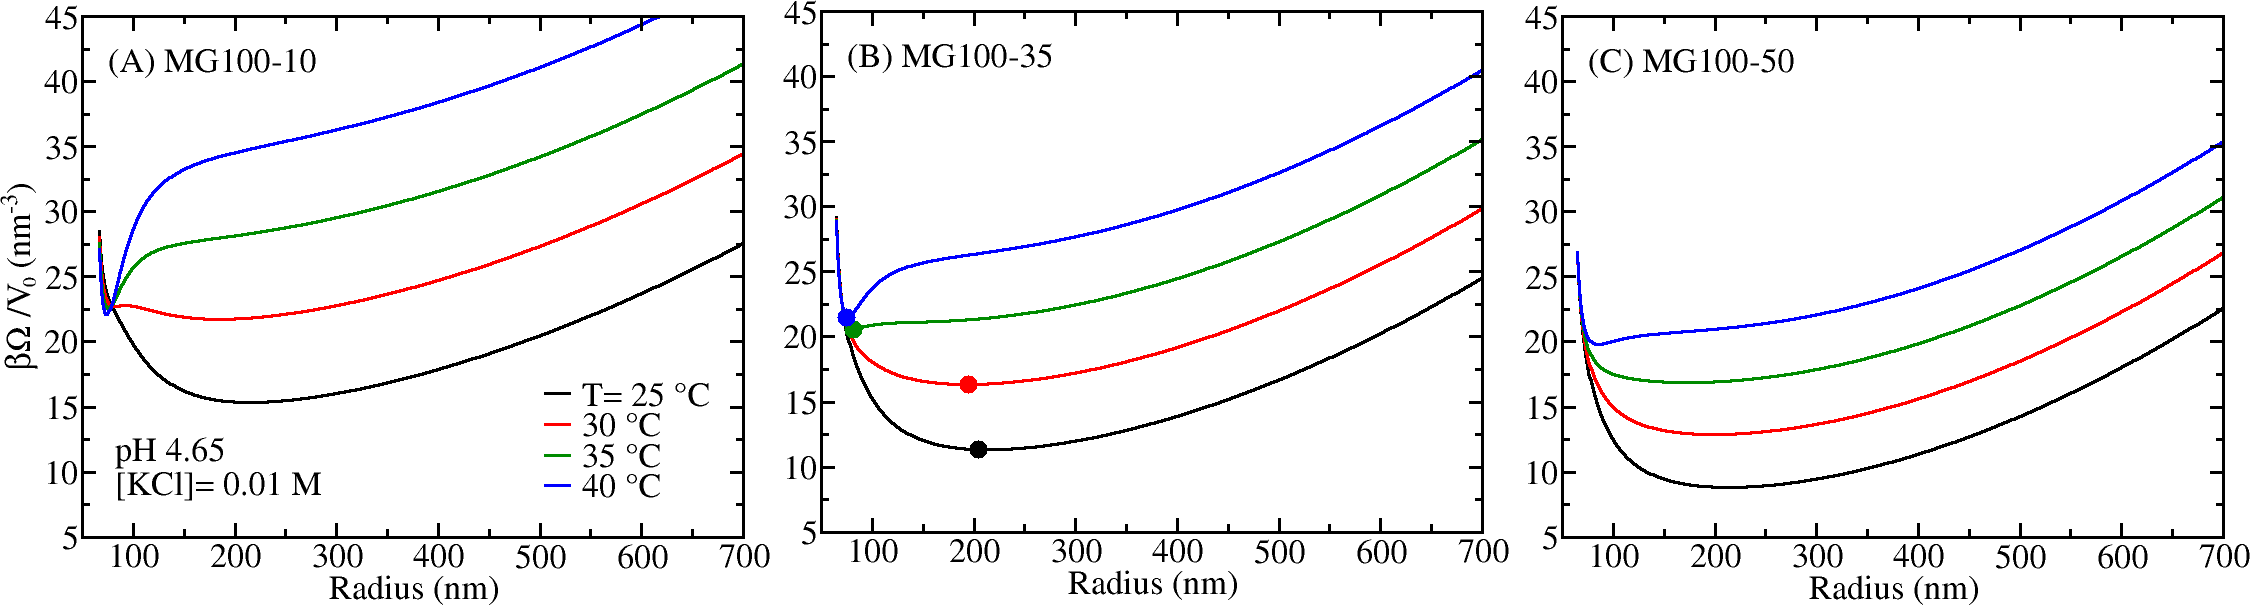
\includegraphics[width=1.\linewidth]{Figures/graph-gel/graph-min.png}
\caption{Potencial termodin\'amico en funci\'on del radio del microgel a diferentes temperaturas, $pH~4.65$ y $cs=10^{-2}M$.
	Cada panel corresponde a un microgel MG100 diferente (longitud de cadena, $n_{ch}=100$) con $10\%$ (A), $35\%$ (B) y $50\%$ (C) MAA.
	Las curvas presentan el potencial termodin\'amico en exceso de la contribuci\'on de la soluci\'on, $\Omega=\Omega_{MG}-\Omega_s$, en algunas unidades convenientes, donde $V_0=\frac{4}{3}\pi R_0^3$ es el volumen de la part\'icula polim\'erica seca.
	En el panel B, los puntos  marcan el radio \'optimo para cada temperatura, que es el m\'inimo local/global de la curva correspondiente (ver tabla \ref{table:optimal-R}).}
\label{fig:graph-min}
\end{figure*}

En este punto, es posible determinar completamente la energí\'i libre de la fase de microgel para cualquier $R$ dado.
Las variables independientes de un c\'alculo son la temperatura, el pH y la concentraci\'on de sal de la soluci\'on en contacto con la fase microgel.
El n\'umero de segmentos en la red de pol\'imero $N_{seg}$, la longitud de la cadena $n_{ch}$ y la fracci\'on de segmentos MAA, $x_{MAA}$, caracterizan completamente el microgel.

We consider microgels with $N_{seg}=10^7$ segments and $n_{ch}=50$, $100$, and $200$, having either $x_{MAA}=0.1$, $0.35$ or $0.5$.
Our goal is to evaluate the effect of increasing or reducing the amount of acidic monomer with respect to poly(NIPAm-\emph{co}-MAA) microgels having $35\%$ MAA, which are typically synthesized in our lab \addcite[Giussi2015,Giussi2020].
These microgels are labeled MG$n_{ch}$-$p_{MAA}$, where $p_{MAA}$ is the percentage of MAA.
For example, MG100-10 is the microgel with  $n_{ch}=100$ and $x_{MAA}=0.1$.


Consideramos microgeles con $N_{seg}=10^7$ segmentos y $n_{ch}=50$, $100$ y $200$, que tienen $x_{MAA}=0,1$, $0,35$ o $0,5$.
El objetivo es evaluar el efecto de aumentar o reducir la cantidad de mon\'omero \'acido con respecto a los microgeles de poli(NIPAm-\emph{co}-MAA) que tienen $35\%$ MAA. % que normalmente se sintetizan en nuestro laboratorio \addcite[Giussi2015 ,Giussi2020].
Estos microgeles est\'an etiquetados como MG$n_{ch}$-$p_{MAA}$, donde $p_{MAA}$ es el porcentaje de MAA.
Por ejemplo, MG100-10 corresponde a un  microgel con $n_{ch}=100$ y $x_{MAA}=0,1$.



To determine the size of the microgel for a given set of conditions, we resource to a graphical minimization procedure.
For each set of conditions (pH, salt, and $T$), we construct $\Omega(R)=\Omega_{MG}(R)-\Omega_{s}(R)$, and find $R_{opt}$, the optimal radius, such that the curve has a local (and global) minimum.
As an example, this procedure is illustrated in figura \ref{fig:graph-min} for MG100 microgels.
The results obtained from the graphical minimization of figura \ref{fig:graph-min} curves are summarized in tabla \ref{table:optimal-R}.

Para determinar el tama\~no del microgel para un conjunto dado de condiciones, recurrimos a una minimizaci\'on gr\'afica del mismo.
Para cada conjunto de condiciones (pH, sal y $T$), construimos $\Omega(R)=\Omega_{MG}(R)-\Omega_{s}(R)$, y encontramos $R_{opt }$, siedo este el radio \'optimo, tal que la curva tenga un m\'inimo local (y global).
Como ejemplo, este procedimiento se ilustra en la figura \ref{fig:graph-min} para microgeles MG100.
Los resultados obtenidos de la minimizaci\'on de las curvas figura \ref{fig:graph-min} se resumen en la tabla \ref{table:optimal-R}.

\begin{table}[!htb]
\centering
\small
  \begin{tabular}{|lccccc|}
   \hline %\multirow{2}{*}{MG100} & 
    %  \multicolumn{4}{c}{Opt. Radius (nm)(MG100)} \\
    	&&   Opt. Radius (nm)(MG100 & && \\
    	\hline
      & {25 $^\circ C$} & {30 $^\circ C$} & {35 $^\circ C$} & {40 $^\circ C$} & {dry, $R_0$} \\
      \hline
    10\% MAA & 215 &  184 &  75  &  74 & 65\\
    35\% MAA &  213 &  193 &  84 & 76 & 64\\
    50\% MAA &  213 & 199 &  172 & 85 & 63\\
    \hline
  \end{tabular}
 \caption{Minimizaci\'on de las curvas de la  figura \ref{fig:graph-min}.
 	Esta tabla resume los radios \'optimos de tres microgeles MG100 a diferentes temperaturas, $pH\,4.65$ y $cs=10^{-2}M$.}
\label{table:optimal-R} 
\end{table}


\subsection{Absroci\'on}
%%%%%%%%%%%%%%%%%%%%%%%%%%%%%%%%%%%%%%%%%%%%%%%%%%%%%%%%%%%%%%%%%%%%%


Para describir la absorci\'on de un analito a la fase de microgel,
el potencial termodin\'amico de la ec. \ref{eq:free-energy} agrega los siguientes t\'erminos:
%
%
%
\begin{align}
\begin{aligned}
\beta&\frac{\Omega_{MG}(R)}{V}= \cdots\\&+ \rho_a\left(\ln\left(\rho_a v_w\right) -1 + \beta\mu^0_a\right) \\
& + \rho_a \sum_\tau n_\tau  \left[g_\tau(\ln g_\tau+ \beta\mu^0_{\tau})\right.\\
&\qquad\left.+(1-g_\tau)(\ln (1-g_\tau)+\beta\mu^0_{\tau H})\right] \\
& +  \left( \rho_a \sum_\tau n_\tau f_\tau q_\tau\right)\beta\psi_{MG}\\
& -\rho_a\beta\mu_a
 -\beta\mu_{H^+} \rho_a \sum_\tau n_\tau g_\tau
\end{aligned}
\label{eq:ads}
\end{align}
%
\noindent La primera l\'inea (lado derecho) representa los grados de libertad de traslaci\'on,
donde $\rho_a$ es la densidad num\'erica del analito y $\mu_a^0$ su potencial qu\'imico est\'andar.
Las siguientes dos l\'ineas describen el equilibrio \'acido-base de las unidades titulables del analito;
el sub\'indice $\tau$ recorre dichas unidades moleculares que tienen un grado de protonaci\'on $g_\tau$ y un volumen $v_\tau$.
El analito tiene $n_\tau$ de estos segmentos;
$\mu^0_{\tau H}$ y $\mu^0_\tau$ son el potencial qu\'imico est\'andar de las especies protonadas y desprotonadas, respectivamente, que se relacionan con la constante de disociaci\'on \'acida:
%
\begin{align}
K^0_{\tau}= e^{\beta\mu^0_{\tau H}-\beta\mu^0_{\tau}-\beta\mu^0_{H^+}}
\end{align}
%

La siguiente l\'inea en la ec. \ref{eq:ads} describe la contribuci\'on del analito a la energ\'ia electrost\'atica, donde $f_\tau$ es el grado de carga de las unidades $\tau$, que es igual a $g_\tau$ si $\tau$ es un grupo b\'asico, o $(1-g_\tau)$ si la unidad es \'acida; $q_\tau$ es la carga de las especies ionizadas.
Los dos \'ultimos t\'erminos dan cuenta del equilibrio qu\'imico entre el microgel y la fase de soluci\'on, donde $\mu_a$ es el potencial qu\'imico del analito.

Adem\'as, la ec. \ref{eq:packing} debe incorporar la fracci\'on total de volumen ocupada por el analito: $\rho_a \sum_\lambda n_\lambda v_\lambda$, donde $\lambda$ recorre todos los tipos de segmentos que forman la mol\'ecula, incluyendo unidades titulables $\{\tau\}\in\{\lambda\}$.
La presencia del analito en la fase de soluci\'on tambi\'en representa contribuciones adicionales al potencial termodin\'amico $\Omega_s$ de ec. \ref{eq:bulk}, que contienen los mismos componentes que ec. \ref{eq:ads}.

De la optimizaci\'on de  $\Omega_{MG}$  se obtiene:
%
\begin{equation}
\frac{f_\tau}{1-f_\tau}=\left(\frac{K^0_\tau}{a_{H^+}}\right)^{\pm 1} e^{-\beta \psi_{MG} q_\tau}
\label{eq:f_ads}
\end{equation}
%
\noindent para el grado de carga de las unidades $\tau$, donde el signo $\pm$ diferencia el caso de un grupo \'acido ($+$) de uno b\'asico ($-$).
Para la densidad del analito obtenemos:
%
\begin{align}
    \begin{aligned}
   \rho_a v_w =&\frac{ \exp{\left(\beta \mu_a - \beta \mu^0_a \right)}}{\prod_\tau \left(1-f_\tau\right)^{n_\tau}}\\
&\quad \cdot\exp{\left(-\beta \pi_{MG} \sum_\lambda n_\lambda v_\lambda \right)} 
    \end{aligned}\label{eq:rho_ads}
\end{align}
%
\noindent where this last equation requires a redefinition of $\mu_a$ and $\mu_a^0$.
Similar expressions to eq. \ref{eq:rho_ads} and eq. \ref{eq:f_ads} are derived for the solution phase.







\begin{figure}[!tb]
\centering
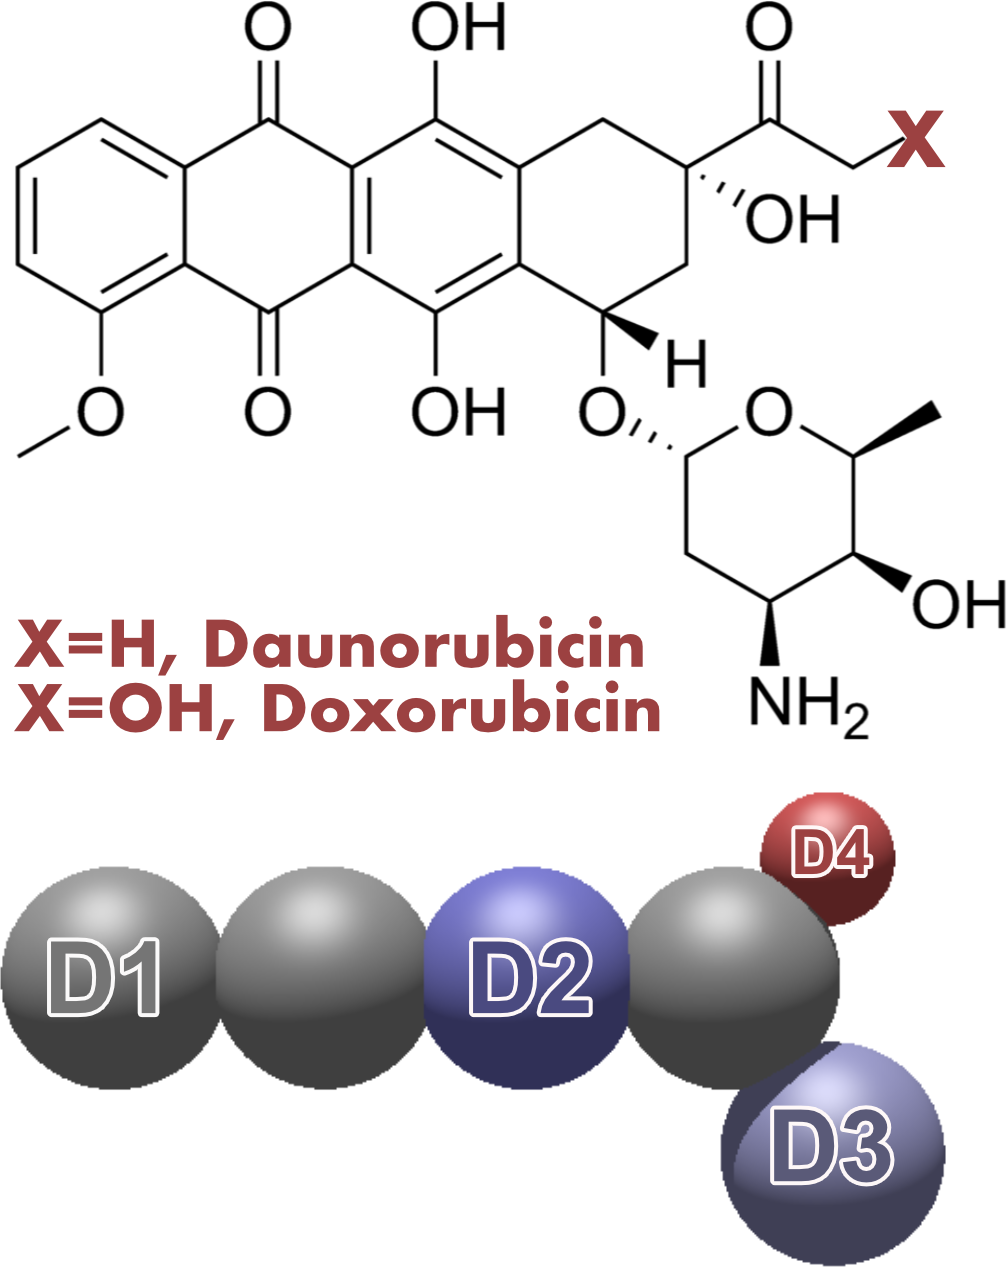
\includegraphics[width=0.35\linewidth]{Figures/graph-gel/dauno-doxo.png}
\caption{Estructura quí\'imica (arriba) y modelo de grano grueso (abajo) aplicado para describir daunorrubicina y doxorrubicina.
	Los segmentos de grano grueso $D1-D4$ se describen en la tabla \ref{table:drugs}.}
\label{fig:dauno-doxo}
\end{figure}



We will consider the absorption of the chemotherapeutic drugs Daunorubicin (Dauno) and Doxorubicin (Doxo) to the P(NIPAm-MAA) microgels under different conditions.
The molecular model applied to describe these analytes is illustrated in figura  \ref{fig:dauno-doxo} and the parametrization is presented in tabla \ref{table:drugs}.\addcite[PerezChavez2020]

Consideraremos la absorci\'on de los f\'armacos quimioterap\'euticos Daunorrubicina (Dauno) y Doxorrubicina (Doxo) a los microgeles P(NIPAm-MAA) en diferentes condiciones.
El modelo molecular aplicado para describir estos analitos se ilustra en la figura \ref{fig:dauno-doxo} y la parametrizaci\'on se presenta en la tabla \ref{table:drugs}.\addcite[PerezChavez2020]

\begin{table}
%\small
%\begin{tabular}{lcS[table-format=-1]S[table-format=0.3]}
\centering
\begin{tabular}{|lccc|}
    \hline
    {CG unit} & {$pKa$} & {$q$ ($e$)} & {$v$ ($\text{nm}^3$)} \\
      \hline
$D1$ & - & 0 & 0.085\\
$D2$ & 7.34 & -1$^\ast$ & 0.085\\
$D3$ & 9.46 & +1$^\ast$ & 0.085\\ 
$D4$ (Doxo) & 8.46 & -1$^\ast$ & 0.035\\
$D4$ (Dauno) & - & 0 & 0.035 \\
    \hline
  \end{tabular}
 \caption{Porpediades moleculares para las distintas unidades de grano grueso usadas para el modelado de las drogas Daunorubicina y Doxorubicina. (ver figura \ref{fig:dauno-doxo}).
\footnotesize ($^\ast$ Para unidades ionizables.)}
\label{table:drugs} 
\end{table}




\section{Resultados y discusi\'on}
%%%%%%%%%%%%%%%%%%%%%%%%%%%%%%%%%%%%%%%%%%%%%%%%%%%%%%%%%%%%%%%%%%%%%



%%%%%%%%%%%%%%%%%%%%%%%%%%%%%%%%%%%%%%%%%%%%%%%%%%%%%%%%%%%%%%%%%%%%%
\subsection{Respuesta al pH y la concentraci\'on de sal}\label{sec:pH_salt}
%%%%%%%%%%%%%%%%%%%%%%%%%%%%%%%%%%%%%%%%%%%%%%%%%%%%%%%%%%%%%%%%%%%%%


\begin{figure}[!ht]
\centering
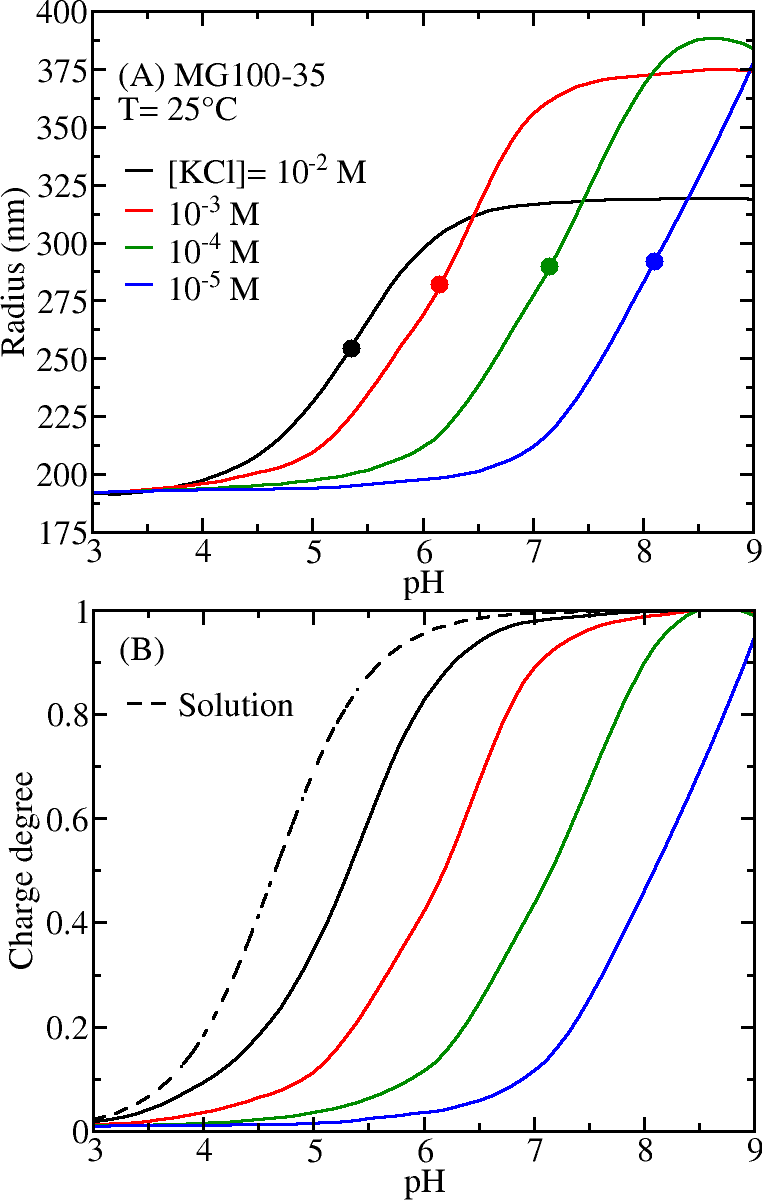
\includegraphics[width=0.5\linewidth]{Figures/graph-gel/R-pH.png}
\caption{Gr\'afico de tama\~no de microgel (A) y grado de carga (B) en funci\'on del pH para soluciones que tienen diferentes concentraciones de sal y $T=25 ^\circ C$.
	Las cadenas de pol\'imero en el microgel MG100-35 son $n_{ch}=100$-long y tienen $35\% $ MAA.
	La curva de línea punteada en el panel B es la disociaci\'on ideal del \'acido metacr\'ilico ($pKa=4.65$).
	Los c\'irculos de color en las curvas del panel A marcan el pKa aparente del microgel.}
\label{fig:R-pH}
\end{figure}

En esta secci\'on, describiremos el comportamiento de los microgeles en respuesta a cambios en la composici\'on de la soluci\'on.
Nos concentramos en temperaturas por debajo de la LCST del PNIPAm;
el efecto de la temperatura se evaluar\'a en \ref{sec:temperature}.


La Figura \ref{fig:R-pH}A muestra el tama\~no del microgel (radio, $R$) en funci\'on del pH para diferentes concentraciones de sal.
Los microgeles P(NIPAm-MAA) se hinchan al aumentar el pH.
A medida que aumenta el pH, un n\'umero creciente de unidades MAA se desprotona y se carga.
Figura \ref{fig:R-pH}B muestra c\'omo la fracci\'on de MAA cargados ($f$: grado de carga; ver ec. \ref{eq:fcharge}) depende del pH de la soluci\'on.
La hinchaz\'on del microgel observada en el panel A a medida que aumenta el pH es la respuesta a las crecientes repulsiones dentro de la red que resultan del aumento de la carga el\'ectrica en el pol\'imero que se ve en el panel B.


El inicio de la transici\'on de hinchamiento se desplaza a valores de pH m\'as altos cuando se reduce la concentraci\'on de sal (ver fig. \ref{fig:R-pH}A).
Las curvas de disociaci\'on de protones del panel B presentan el mismo desplazamiento a pHs m\'as altos, con respecto al comportamiento ideal de un mon\'omero MAA aislado en soluci\'on diluida.
El pKa aparente de un microgel es el pH al que se desprotonan la mitad de los segmentos MAA;
cuantifica el comportamiento de carga del microgel, fig. \ref{fig:R-pH}B, pero tambi\'en la transici\'on de expansi\'on como vemos en el panel A (ver circulos en $pH=pKa$).
Los pKa aparentes de la fig. \ref{fig:R-pH}B se muestran en la tabla \ref{table:pKa_app}.

\begin{table}[!htb]
\small
  \begin{tabular}{|cc|}
    \hline
      [NaCl] (M)&  pKa app. ($25 ^\circ C$)  \\
      \hline
    $10^{-5}$ & 8.10  \\
    $10^{-4}$ & 7.15 \\
    $10^{-3}$ & 6.15 \\
    $10^{-2}$ & 5.35 \\
    %\azul $10^{-1}$ & \azul 4.80 \\
    ideal (pKa) &  $4.65$  \\
    \hline
  \end{tabular}
 \caption{ pka's aprente de la fig. \ref{fig:R-pH} para un gel MG100-35 a $25 ^\circ C$.}
\label{table:pKa_app} 
\end{table}


Una concentraci\'on relativamente alta de iones de sal dentro del microgel da como resultado la detecci\'on de las repulsiones electrost\'aticas entre los segmentos MAA cargados; estas interacciones repulsivas se vuelven de corto alcance.
Cuando el pH de la soluci\'on aumenta, la disociación de MAA sucede sin un alto costo energ\'etico de repulsiones electrost\'aticas.
En estas condiciones, la desprotonaci\'on de MAA, inducida por la energ\'ia qu\'imica libre (equilibrio \'acido-base), se aproxima al comportamiento ideal o de soluci\'on diluida (compare los casos de alta [sal] con la curva de l\'inea punteada en la fig. \ref{fig:R -pH}B).



Por el contrario, el efecto de apantallamiento se debilita y las repulsiones electrost\'aticas dentro de la red son de mayor alcance para soluciones con baja concentraci\'on de sal.
Incluso si aparecen pocas cargas distantes en la red, interactuar\'an entre s\'i.
Para reducir la contribuci\'on energ\'etica de tales repulsiones electrost\'aticas, es significativamente menos probable que las unidades MAA se carguen en condiciones de baja salinidad;
el pKa aparente aumenta.
El precio a pagar en cambio es aumentar la energ\'ia química libre, cuya contribuci\'on se minimiza cuando el grado de protonaci\'on es ideal.



\begin{figure*}[!htb]
	\centering
	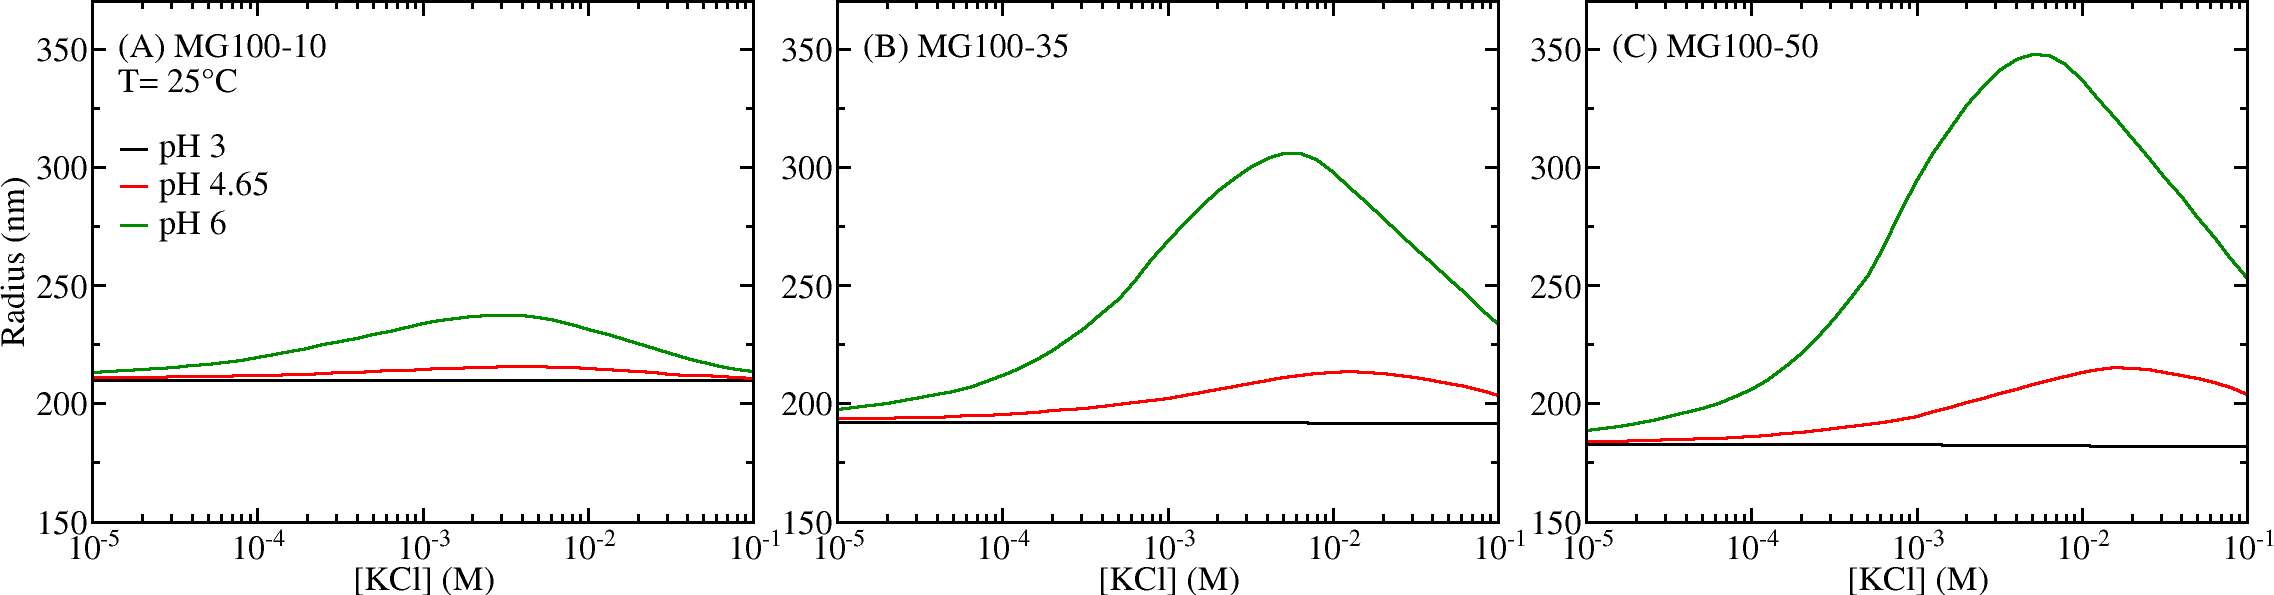
\includegraphics[width=1\linewidth]{Figures/graph-gel/R-cs.png}
	\caption{Gr\'afico del tama\~no del microgel en funci\'on de las concentraciones de sal para diferentes soluciones de pH y $T=25 ^\circ C$.
		Los paneles corresponden a microgeles MG-100 (longitud de cadena, $n_{ch}=100$) que tienen fracciones MAA: $10\%$ (A), $35\%$ (B) y $50\%$ (C).}
	\label{fig:R-cs}
\end{figure*}

La figura \ref{fig:R-cs} ilustra c\'omo el tama\~no de los microgeles de P(NIPAm-MAA) depende de la concentraci\'on de sal para diferentes valores de pH.
A una salinidad relativamente alta, estos microgeles se hinchan con el aumento de la concentraci\'on de sal, lo que es consistente con los resultados de dispersi\'on de luz din\'amica (DLS) de \addcite[citet:Wong2009] para microgeles P(NIPAm-MAA) y concentraciones de NaCl en el rango de $0.1-0.5 M$.

Las curvas de la Figura \ref{fig:R-cs} muestran un comportamiento reentrante, en el que el tama\~no primero aumenta y luego disminuye al aumentar la concentración de sal.
Esta respuesta no monot\'onica es m\'as prominente cuando la carga del pol\'imero aumenta debido a un mayor contenido de pH o MAA (compare diferentes paneles de firgura \ref{fig:R-cs}).



Se han informado transiciones de hinchamiento-deshinchamiento con concentraciones de sal variables para una variedad de sistemas polim\'ericos reguladores de carga.
El grosor de las capas de poli\'acidos d\'ebiles anclados es una funci\'on no monot\'onica de la concentraci\'on de sal de la soluci\'on seg\'un lo predicho por la teor\'ia del campo medio autoconsistente \addcite[Israels1994,Lyatskaya1995,Zhulina1995,Gong2007], que ha sido confirmada por resultados experimentales \addcite [Wu2007].
De manera similar, los resultados te\'oricos predicen que el tama\~no de los polielectrolitos d\'ebiles ramificados en estrella muestra un m\'aximo en funci\'on de la concentraci\'on de sal en la soluci\'on \addcite[Borisov1998,KleinWolterink2002];
Tambi\'en se ha predicho que el espesor de las pel\'iculas de poliácidos d\'ebiles entrecruzados mostrar\'a este comportamiento de hinchamiento reentrante \addcite[Longo2014JCP].

Se ha predicho una transici\'on deshinchaz\'on a hinchaz\'on impulsada por la sal para los nanogeles de polielectrolitos fuertes \addcite[jha2012understanding];
este comportamiento, en el caso de los polielectrolitos quencheados, se atribuy\'o a los efectos de volumen excluidos de los iones absorbidos a altas concentraciones de sal.
M\'as relevante para nuestro estudio, se predijo te\'oricamente una transici\'on de hinchaz\'on a colapso reentrante para microgeles sensibles al pH y al calor \addcite[polotsky2013collapse].
\addcite[citet:polotsky2013collapse] explica que el aumento de la concentraci\'on de sal primero promueve la disociaci\'on de carga de los grupos \'acidos d\'ebiles hasta que se alcanza la saturaci\'on cuando el grado de disociaci\'on alcanza el valor ideal.
M\'as all\'a de este punto, el aumento de la concentraci\'on de sal de la soluci\'on solo mejora la detecci\'on de las repulsiones electrost\'aticas y, por lo tanto, el microgel se deshincha.
Experimentalmente, \addcite[citet:CaprilesGonzalez2008] inform\'o el hinchamiento no mon\'otónico de los microgeles de poli(NIPAm-\emph{co}-AA) (P(NIPAm-AA)) en funci\'on de la concentraci\'on de NaCl usando DLS.

\begin{figure}[!tb]
	\centering
	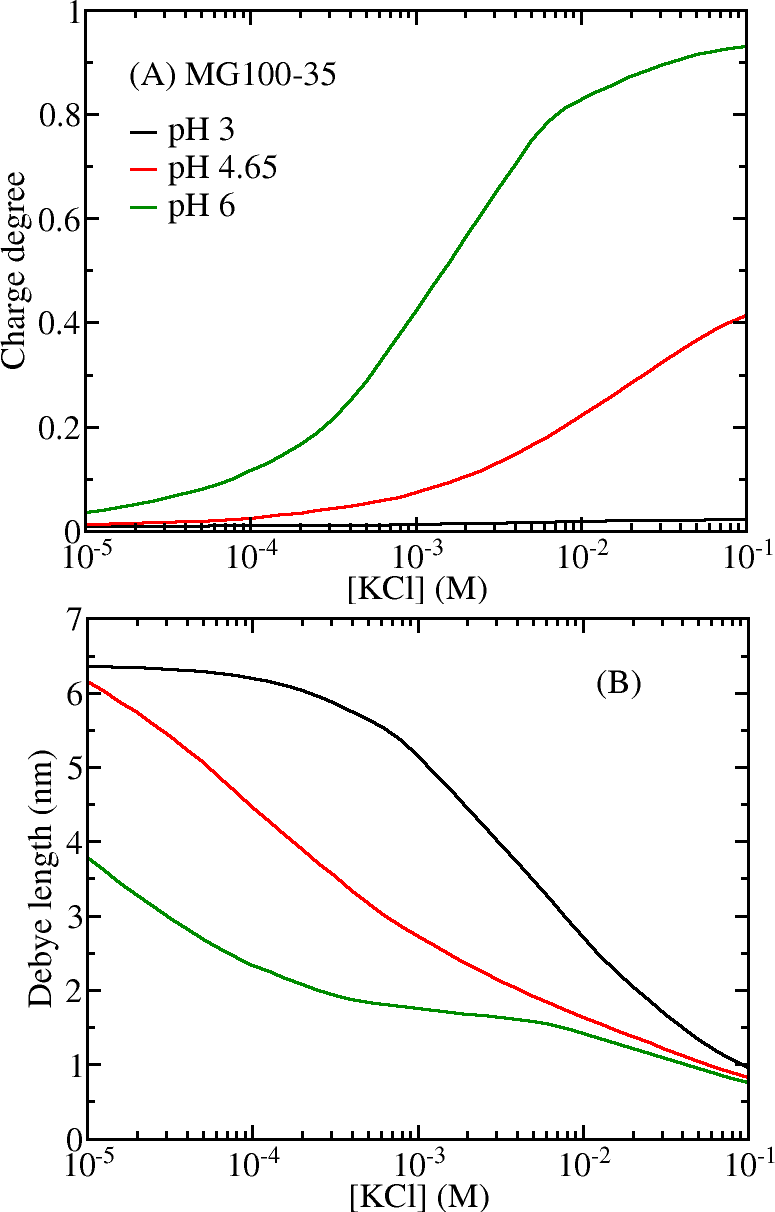
\includegraphics[width=0.5\linewidth]{Figures/graph-gel/f-cs.png}
	\caption{Plots of MAA degree of charge (A) and Debye length (B) inside MG100-35 microgels as a function of salt concentration for different pH values.
		These results correspond to the conditions of figura \ref{fig:R-cs}B.}
	\label{fig:f-cs}
\end{figure}




Increasing salt concentration of the solution has two opposite effects on the microgel properties.
On the one hand, it enhances the screening of charge interactions as more ions partition inside the gel; electrostatic repulsions between charged MAA monomers are increasingly shielded.
The effective reach of these repulsions shortens, favoring deswelling.
On the other hand, this shielding allows for further deprotonation of MAA monomers, promoted by the acid-base equilibrium.
Charge dissociation favors swelling to reduce electrostatic repulsions.


Figura \ref{fig:f-cs} illustrates this dual effect of increasing the concentration of salt in the bulk solution, which leads to the swelling-deswelling behavior.
Panel A shows that the microgel charge increases monotonically with [salt].
In panel B, we use the Debye length to quantify extent of electrostatic interactions %(see \cref*{si:eq:debye_length} in the \supp).
The effective reach of these interactions shortens inside the microgel as the salt concentration increases.
Incidentally, figura \ref{fig:f-cs}A shows that when $pH~3$ the charge inside the polymer network is negligible, which results in no appreciable swelling in figura \ref{fig:R-cs}B.



Our theory requires the interior of the microgel to be charge neutral.
\addcite[citet:Claudio2009] demonstrated that this is a reasonable approximation when the microgel is larger than $R=125\,\text{nm}$ having 50\% of monomers charged.
The P(NIPAm-MAA) microgels of this work are larger than that size under most conditions, particularly when pH is above the apparent pKa and most MAA groups are deprotonated. 
Moreover, salt ions absorb inside the microgel to reinforce such constraint, which allows MAA segments to deprotonate and become electrically charged.
We describe this effect as the screening of the electrostatic repulsions between MAA groups, which is a functional concept that allows for a clear interpretation many features of these microgels behavior. %\cite{Longo2011}.

\subsection{Temperature Response}\label{sec:temperature}
%%%%%%%%%%%%%%%%%%%%%%%%%%%%%%%%%%%%%%%%%%%%%%%%%%%%%%%%%%%%%%%%%%%%%

\begin{figure*}[!htb]
	\centering
	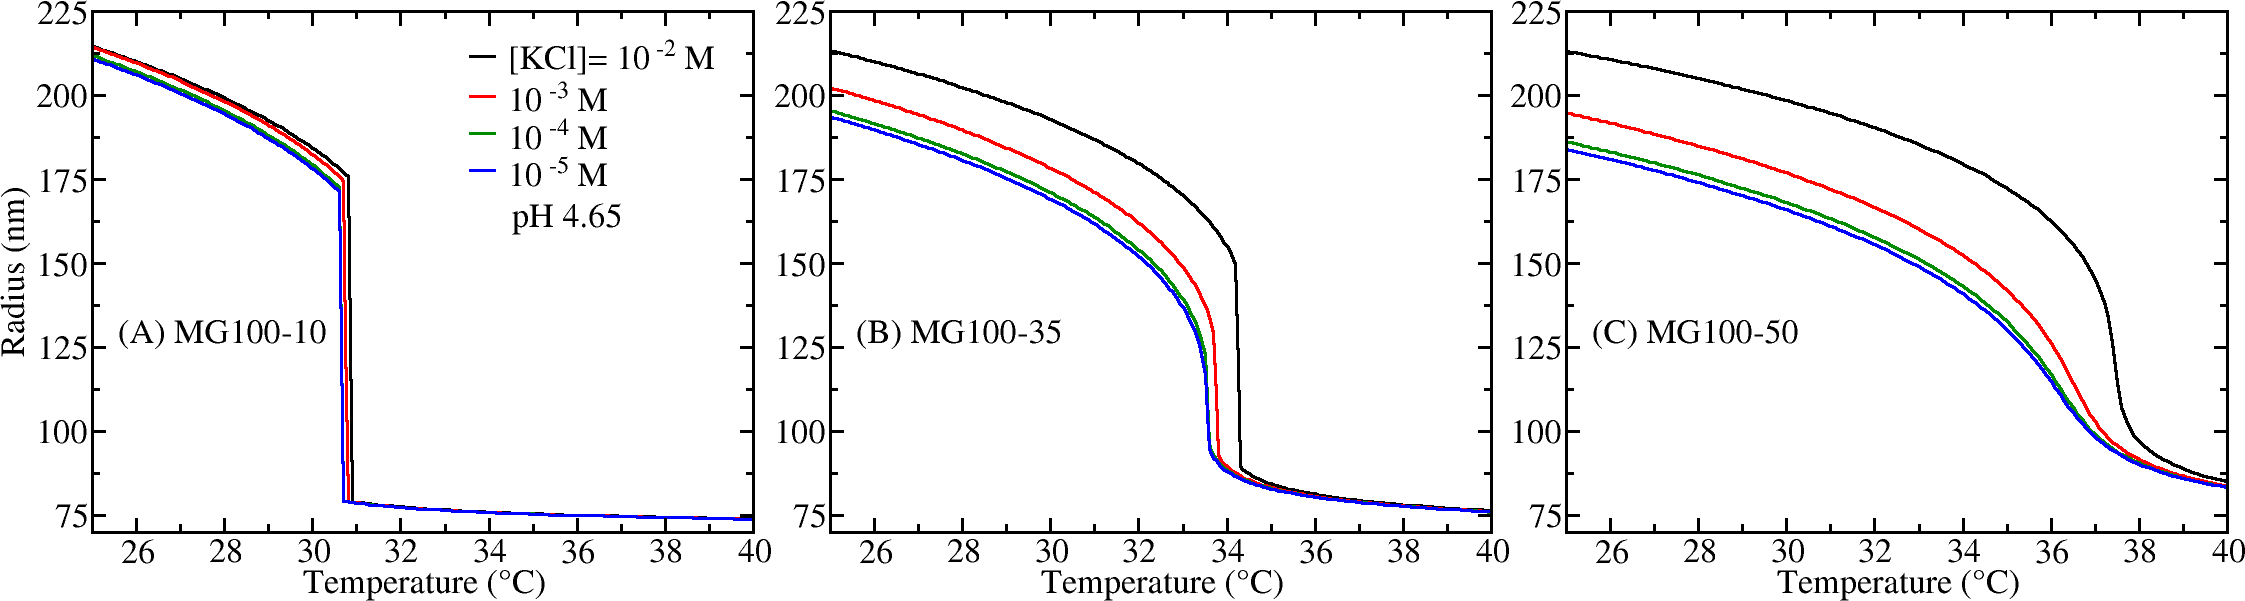
\includegraphics[width=1\linewidth]{Figures/graph-gel/R-T.png}
	\caption{Plot of the microgel size as a function of temperature for different solution salt concentrations and $pH~4.65$.
		Panels correspond to MG-100 microgels (chain length, $n_{ch}=100$) having different MAA fractions: $10\%$ (A), $35\%$ (B), and $50\%$ (C).}
	\label{fig:R-T}
\end{figure*}




In this section, we consider the response of P(NIPAm-MAA) microgels to temperature changes under different conditions.
Each panel of figura \ref{fig:R-T} shows the size of a different MG-100 microgel as a function of temperature for various salt concentrations.
At low temperature, these microgels display a relatively swollen state, while a collapsed (high polymer density) state takes place at high temperatures.



This latter state occurs because PNIPAm becomes hydrophobic above its LCST, leading to the expulsion of water and the collapse of the microgel structure.\addcite[sbeih2019structural]
The microgel size in this state is roughly independent of salt concentration or pH, and relatively close to that of the dry particle (see tabla \ref{table:optimal-R}).


On the other hand, the swollen state is dominated by the electrostatic repulsions between charged MAA segments and the adsorption of salt counterions, as discussed in sec. \ref{sec:pH_salt}.
Microgel size and charge are both monotonously decreasing functions of 
the temperature.
The swollen state is characterized by a larger degree of charge %(see \cref*{si:fig:f-T} in the \supp).
Indeed, the swollen to collapsed VPT is accompanied by a transition in the degree of charge of MAA segments.


\begin{figure}[!htb]
	\centering
	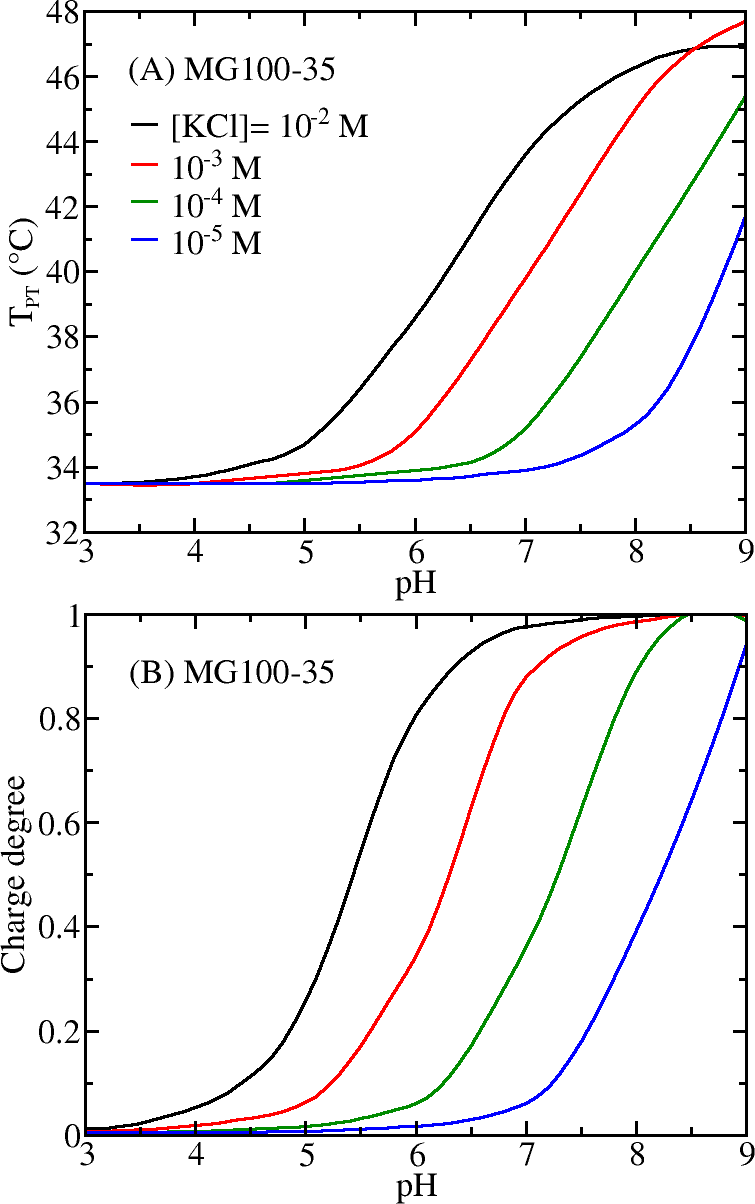
\includegraphics[width=0.5\linewidth]{Figures/graph-gel/Tpt-pH.png}
	\caption{Plots showing the volume transition temperature $T_{PT}$ (A) and the fraction of charged MAA at this temperature (B) as a function of pH for different salt concentrations.
		This P(NIPAm-MAA) microgel has $n_{ch}=100$ chain length and $35\%$ MAA.}
	\label{fig:Tpt-pH}
\end{figure}



Under most but not all conditions, the transition between these two states of the microgel is sharp, occurring in a narrow range around a well defined temperature ($T_{pt}$).
Comparing the different panels of figura \ref{fig:R-T}, we see that increasing the MAA content of the microgels leads to a smoother transition around $T_{pt}$.



Figura \ref{fig:Tpt-pH}A shows that the $T_{pt}$ increases with pH and salt concentration.
These results are consistent with DLS experiments showing that the VPTT of P(NIPAm-MAA) microgels increases with pH \addcite[Kleinen2008], which has also been observed for P(NIPAm-AA) microgels \addcite[CaprilesGonzalez2008].
We have defined $T_{pt}$ as the inflection point of the $R(T)$ curves of figura \ref{fig:R-T} between the swollen and collapsed states \addcite[Kratz2001].






Panel B of figura \ref{fig:Tpt-pH} shows the degree of charge of MAA segments at the $T_{pt}$.
There is a clear correlation between the dependence of $T_{pt}$ with the pH and salinity and the state of charge of the microgel at the VPT conditions.
The transition temperature increases with pH and salt concentration as does the charge of polymer network.

As opposed to this behavior, The VPTT of permanently charged PNIPAm-based microgels decreases with salt concentration\addcite[Lopez2020].
In this case, the charge of the polymer remains constant while the incorporation of salt ions only weakens the electrostatic repulsions between these charges.







\begin{figure}[!tb]
	\centering
	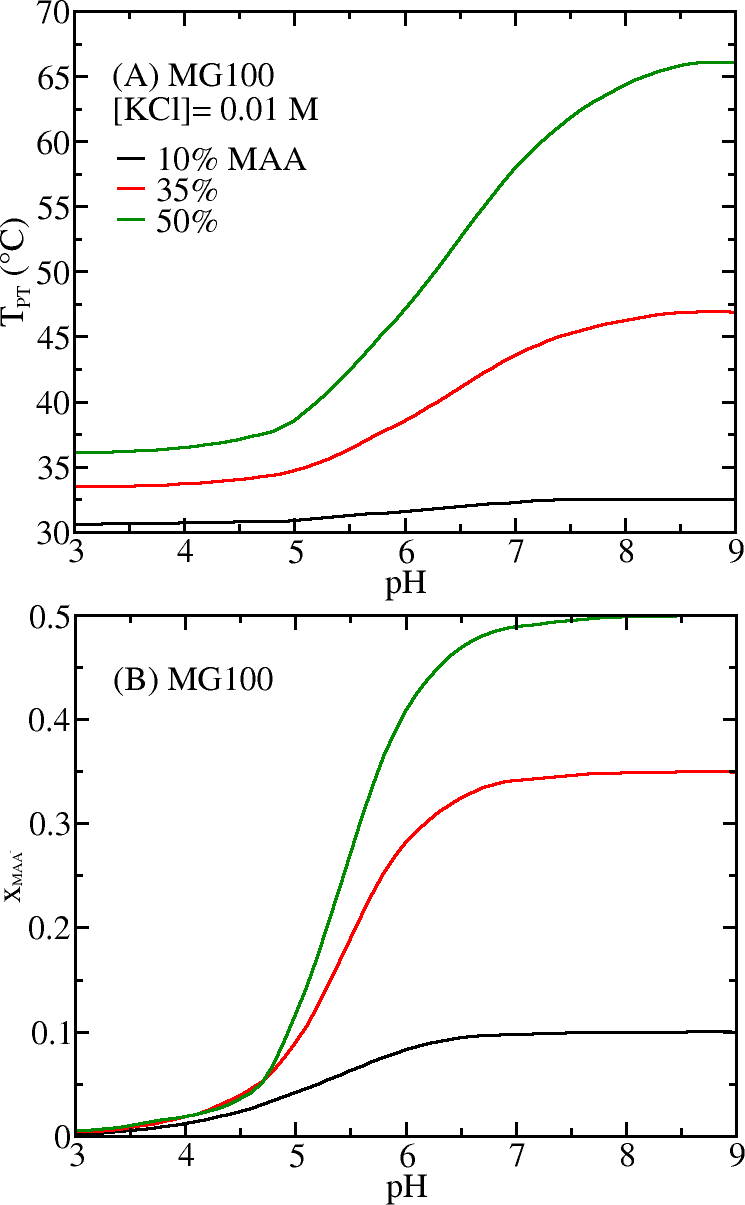
\includegraphics[width=0.5\linewidth]{Figures/graph-gel/Tpt-pH_MAA.png}
	\caption{(A) Plot of transition temperature $T_{PT}$ as a function of pH for MG-100 microgels (polymer chain length, $n_{ch}=100$ segments) having different MAA contents; $[salt]=0.01 M$;
		(B) Fraction of charged segments $x_{MAA^-}=\frac{N_{MAA^-}}{N_{seg}}$ as a function of pH for the same conditions of panel A (\emph{i.e.}, at the $T_{pt}$); $x_{MAA^-}$ is proportional to the total charge of the polymer; $N_{seg}$ is the same for all microgels.}
	\label{fig:Tpt_MAA}
\end{figure}



The results of figura \ref{fig:Tpt-pH} show that the transition temperature is controlled by the amount of charge inside the microgel.
Indeed, increasing MAA content has the same effect of displacing the VPTT to higher values, as seen in figura  \ref{fig:Tpt_MAA}A.
Once again this behavior results from a more charged polymeric structure.
To compare the state of charge of microgels with different MAA contents, we use the total fraction of charged monomers:
%
\begin{equation}
x_{MAA^-}=\frac{N_{MAA^-}}{N_{seg}}=f x_{MAA}
\end{equation}
%
\noindent where $N_{MAA^-}$ is the number of deprotonated MAA segments; all other quantities have been defined in sec. \ref{sec:theory};
$x_{MAA^-}$ is proportional to the total charge of the microgel network, and
because all microgels have the same total number of segments, the proportionally constant is the same for all MAA contents considered.
figura \ref{fig:Tpt_MAA}B shows that there is a clear correlation between the $T_{pt}$ and the total charge of the microgel (given by $x_{MAA^-}$) when changing pH or the MAA content of the polymer.

%%%%%%%%%%%%%%%%%%%%%%%%%%%%%%%%%%%%%%%%%%%%%%%%%%%%%%%%%%%%%%%%%%%%%
\subsection{Effect of Degree of Crosslinking}
%%%%%%%%%%%%%%%%%%%%%%%%%%%%%%%%%%%%%%%%%%%%%%%%%%%%%%%%%%%%%%%%%%%%%


\begin{figure*}[!tb]
	\centering
	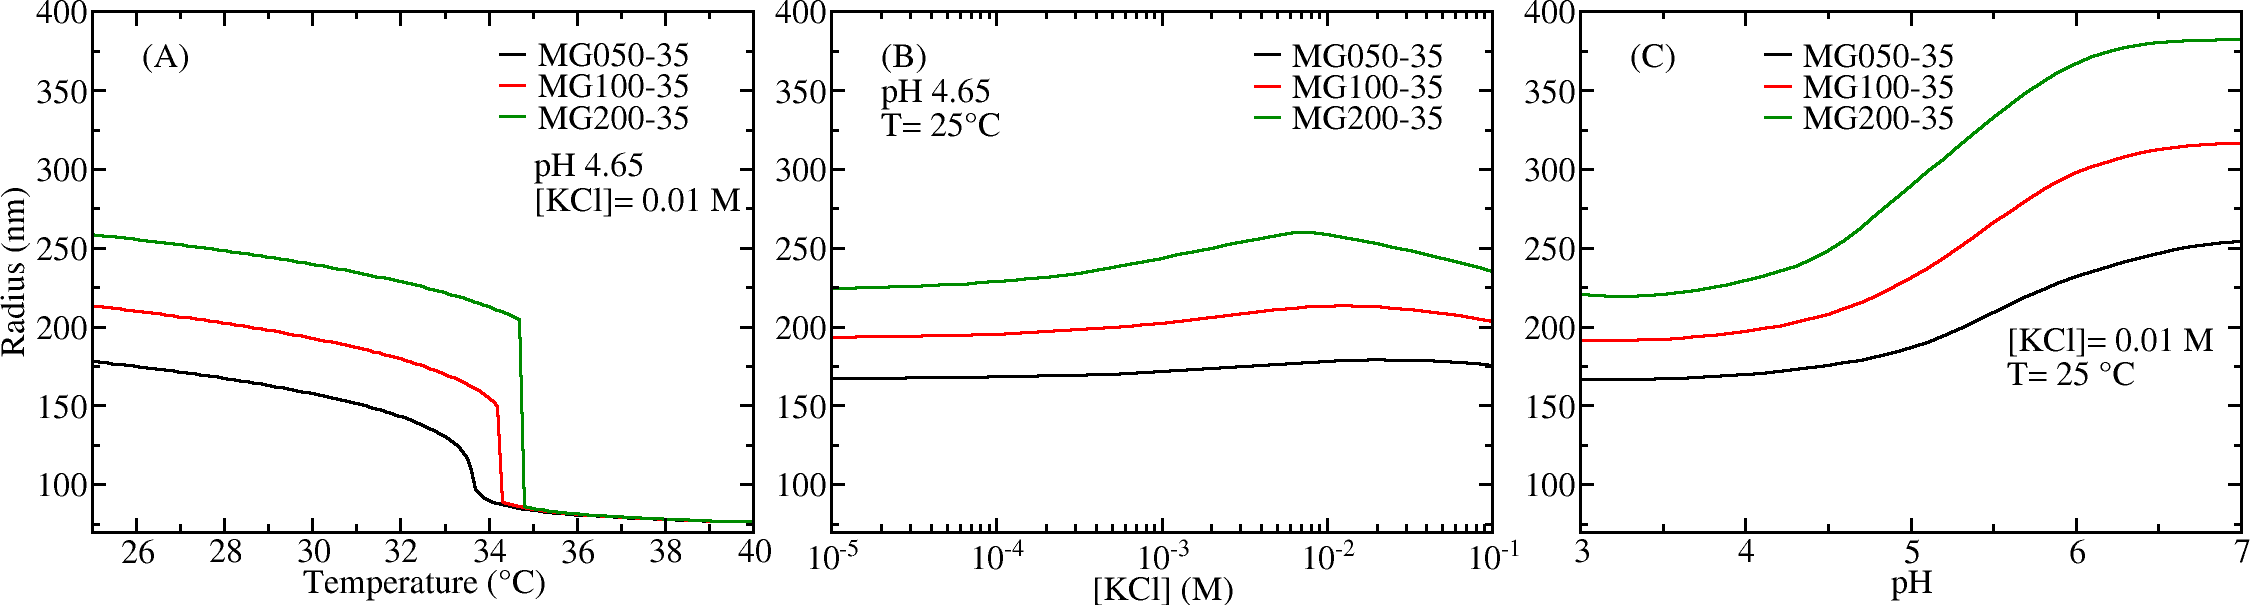
\includegraphics[width=1\linewidth]{Figures/graph-gel/R-all_xlink.png}
	\caption{Plot of microgel size as a function of temperature, salt concentration and pH (panels A, B and C respectively). 
		Different curves correspond to microgels with $50$ (MG050), $100$ (MG100) and $200$ (MG200) segments per polymer chain, all having $35\%$ MAA.}
	\label{fig:R_xlink}
\end{figure*}









Next we analyze how the degree of crosslinking of the polymer network affects the behavior described in the previous sections. 
We have considered microgels with $50$, $100$ and $200$ segments per chain.
Overall, these particles have the same total number of segments.
Figure \ref{fig:R_xlink} shows the response of $35\%$ MAA microgels to changes in temperature (panel A), salt concentration (B), and pH (C).



Microgels with lower degree of crosslinking (higher number of segments per chain) display greater swelling.
This behavior of P(NIPAm-MAA) microgels has been experimentally confirmed\addcite[khan2013preparation].
Qualitatively, the response to salt concentration and pH is similar (panels B and C of figura \ref{fig:R_xlink}, respectively) for all chain lengths considered.
An interesting observation is that decreasing the crosslinking degree leads to a more sharp volume transition when the temperature increases (figura \ref{fig:R_xlink}A);
in addition, $T_{pt}$ increases.
Our results are consistent with the works of \addcite[citet:li1989study] and \addcite[citet:wu1997volume] that reported a change in the volume transition of NIPAm from continuous to discontinuous as the concentration of crosslinker in the synthesis decreases.



In figura \ref{fig:R_xlink} we also see that increasing chain length (decreasing the degree of crosslinking) displaces the $T_{pt}$ to higher temperatures.
This is consistent with the UV spectroscopy results of \addcite[citet:Lee2008] for P(NIPAm-AA) microgels.
This behavior occurs for all the range of conditions explored in this work %(see \cref*{si:fig:Tpt-pH_nch} in the \supp, for example).


The force constant of the elastic contribution to the free energy is inversely proportional to the chain length $n_{ch}$ (see eq. \ref{eq:free-energy}).
By lowering the degree of crosslinking, the more flexible microgel swells, which allows for a higher degree of charge on the polymer network.
In consequence, a higher temperature is required to induce collapse of the polymer network.
We have shown that $T_{pt}$ is strongly correlated to the degree of charge.


The presence of acidic units accentuates the dependence of $T_{pt}$ on chain length because it incorporates protonation equilibrium to the game, but this behavior is intrinsic to the balance between hydrophobic interactions and network elasticity.
Indeed, the transition temperature of pure PNIPAm microgels increases with chain length as well, though the effect is significantly weaker in the absence of MAA segments.



%%%%%%%%%%%%%%%%%%%%%%%%%%%%%%%%%%%%%%%%%%%%%%%%%%%%%%%%%%%%%%%%%%%%%
\subsection{Drug Absorption}
%%%%%%%%%%%%%%%%%%%%%%%%%%%%%%%%%%%%%%%%%%%%%%%%%%%%%%%%%%%%%%%%%%%%%




Multiresponsive microgels are regarded as excellent candidates for the development of functional drug delivery vehicles.
For example, it is known that the extracellular pH of tumor tissue is lower than that of healthy tissue \addcite[Gerweck1996], which makes pH-responsive microgels
ideal for the local administration of anticancer drugs\addcite[Dadsetan2013].
%The tissue-like environment inside microgels can provide stability to encapsulated peptides or proteins and help them retain activity upon release\cite{Malmsten2010}.
Moreover, to achieve intestinal drug delivery via the oral route,
pH-sensitive microgels based on MAA have been extensively studied in by Peppas \emph{et al.} as intelligent carriers that can operate using the different acidity levels along the digestive tract and prevent drug degradation in the stomach\addcite[TorresLugo2002,Carr2010,DuranLobato2014,Sharpe2018].







In this section, we evaluate the ability of P(NIPAm-MAA) microgels to incorporate two chemotherapeutic drugs.
In particular we investigate the best conditions for drug encapsulation under lab conditions.
We consider Doxorubicin (Doxo) and Daunorubicin (Dauno) that are two of the most important anthracyclines used in chemotherapy to treat a wide range of cancers.\addcite[Panis2012,Carvalho2009,aubel1984daunorubicin,come1999dual]
These therapeutics can be followed using fluorescence and adsorbance, which makes them attractive from a research standpoint.\addcite[Serpe2005,ThanHtun2009,PerezChavez2020] 
In addition, these drugs are positively charged under most conditions, which can facilitate their encapsulation within anionic polymer microgels.\addcite[Li2019]]
\addcite[citet:Serpe2005] have studied the thermally activated uptake and release of Doxo from layer-by-layer films of P(NIPAm-AA) microgels and poly(allylamine hydrochloride).
More recently, using time-lapse nuclear magnetic resonance, \addcite[citet:MartinezMoro2020] have described the interaction between Doxo and P(NIPAm-MAA) microgels under different conditions.  



\begin{figure}[!tb]
	\centering
	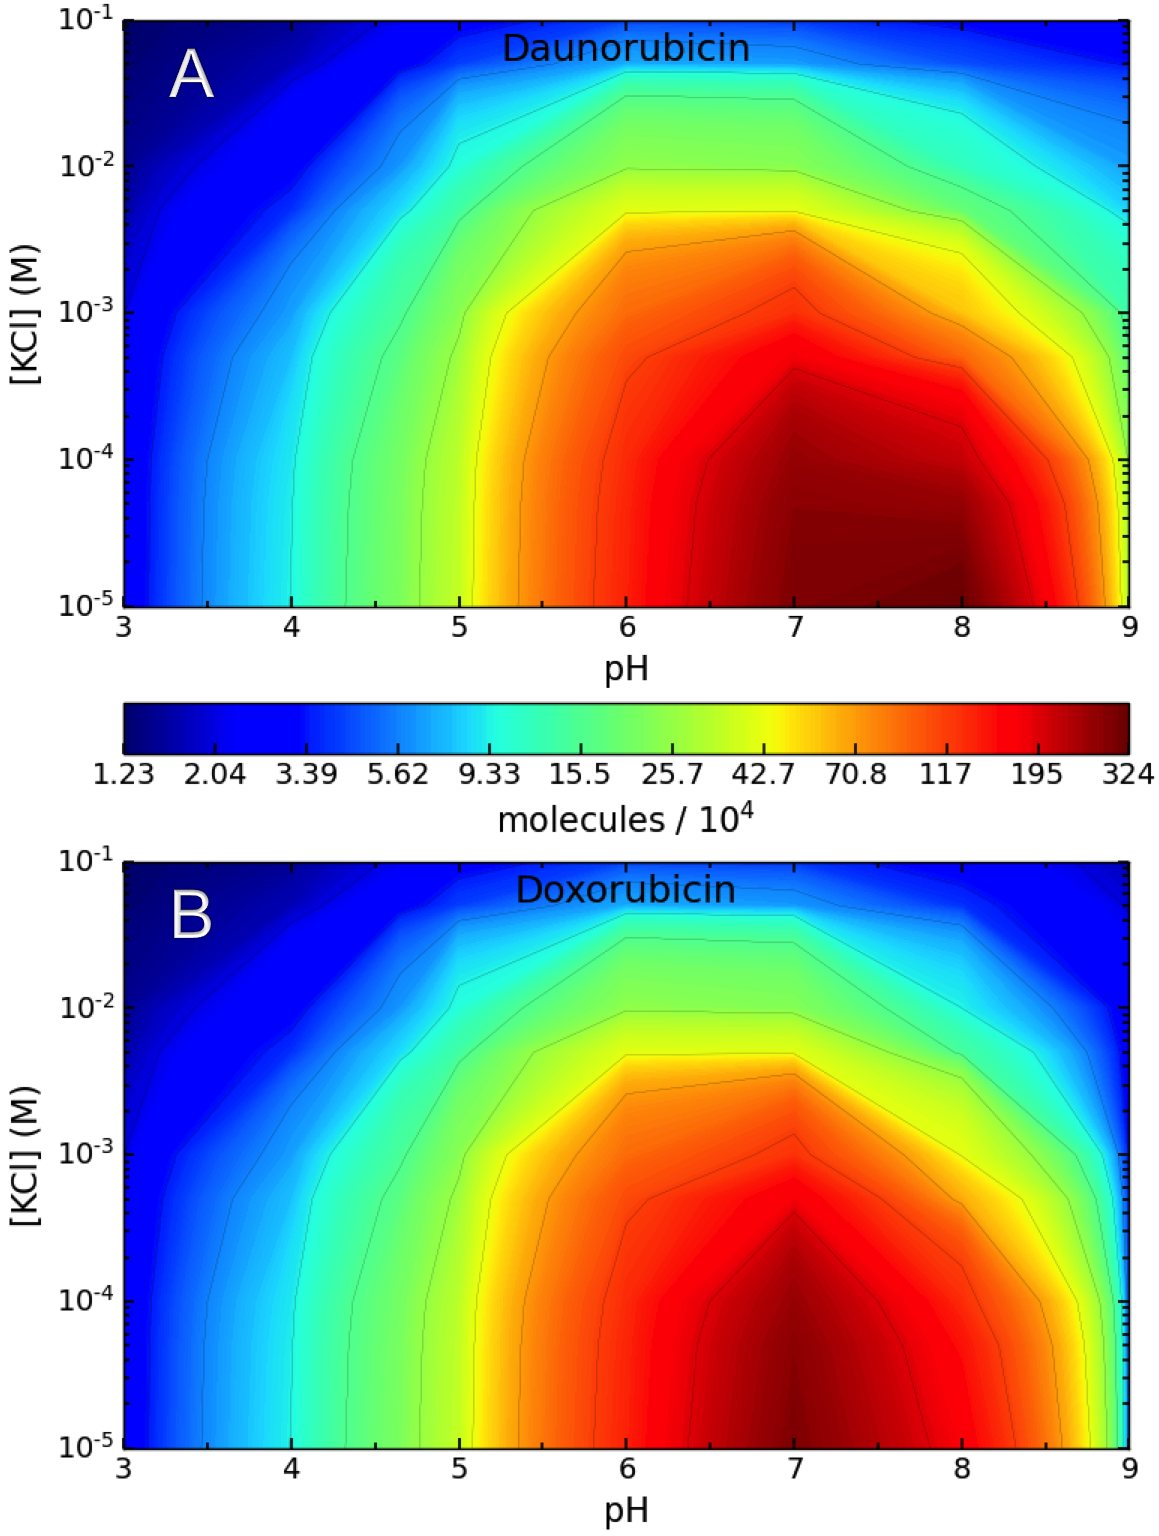
\includegraphics[width=0.55\linewidth]{Figures/graph-gel/drug_ads.png}
	\caption{Color maps showing the number of microgel-absorbed (A) Daunorubicin and (B) Doxorubicin molecules as a function of the solution pH and salt concentration.
		The solution drug concentration is $1mM$ and $T=25 ^\circ C$.
		the P(NIPAm-MAA) microgel has $n_{ch}=100$ chain length and $35\%$ MAA (MG100-35).}
	\label{fig:drug_ads}
\end{figure}




Figura \ref{fig:drug_ads} shows the number of Dauno (panel A) and Doxo (panel B) molecules inside the microgel as a function of the solution salt concentration and pH.
Clearly, the best conditions for encapsulation of these therapeutic drugs correspond to low salt concentration and pH $6-8$.
Lowering salt concentration favors absorption.
Both Dauno and Doxo have $+1$ net charge at acidic and neutral pH %(see \cref*{si:fig:drugs-Q} in the \supp).
As a result, their absorption has to compete with that of potassium ions to neutralize the negative charge of the polymer network.\addcite[PerezChavez2020].
Figura \ref{fig:f-cs} shows that in the absence of a dissolved drug the microgel charge decreases with lowering the salt concentration, which seems to conflict with the enhanced absorption seen in figura \ref{fig:drug_ads} under these conditions.
However, upon drug absorption the degree of charge of MAA segments increases significantly, particularly under low salt conditions %(see \cref*{si:fig:f-cs_doxo}).
Note also that this behavior is particularly associated with the relatively high drug concentration considered in this work ($1\,$mM).

The fraction of negatively charged MAA segments in the polymer increases with pH, which explains why Dauno/Doxo absorption increases as well (acidic conditions).
Under alkaline conditions, however, the net positive charge of these drugs decreases with increasing pH, which disfavors absorption.
As a result, Dauno/Doxo absorption is a nonmonotonic function of pH.



In our model, the isoelectric points of Dauno and Doxo are $8.4$ and $7.9$, respectively% (see \supp \cref*{si:fig:drugs-Q}).
Figura \ref{fig:drug_ads} shows that the absorption of both molecules can be significant around and above these pH values.
In other words, there is considerable absorption of negatively charged molecules inside the similarly charged polymer network.
Although, indeed these molecules are negatively charged in the solution phase, absorption occurs because the pH drops inside the microgel, allowing the drugs to regulate its electric charge and remain positively charge inside the microgel %(\cref*{si:fig:drugs-pH}, \supp).


The lower isoelectric point of Doxorubicin is due to the deprotonation of its substituent hydroxyl group (see $D4$ in figura \ref{fig:dauno-doxo} and tabla \ref{table:drugs}).
As a result of this additional negative charge under alkaline conditions, the pH range of significant adsorption is slightly wider for Daunorubicin.